\documentclass{beamer}
\usepackage[french]{babel}
\usepackage{hyperref}
\usepackage{graphicx}
\usepackage{amsmath,amssymb}
\usepackage{tabularx}
\usepackage{booktabs}
\usepackage[compatibility=false]{caption}
\usepackage[toc,page]{appendix}
\usepackage{minted}

\makeatletter
  \def\beamer@calltheme#1#2#3{%
    \def\beamer@themelist{#2}
    \@for\beamer@themename:=\beamer@themelist\do
    {\usepackage[{#1}]{\beamer@themelocation/#3\beamer@themename}}}

  \def\usefolder#1{
    \def\beamer@themelocation{#1}
  }
  \def\beamer@themelocation{}


\newcolumntype{Y}{>{\centering\arraybackslash}X}

\usefolder{../theme}
\usetheme[numbering=fraction,block=fill,progressbar=frametitle]{metropolis} %Use metropolis theme

\definecolor{bg}{rgb}{0.95,0.95,0.95}
\setminted{bgcolor=bg,fontsize=\scriptsize,autogobble,mathescape,breaklines,tabsize=2}
\setmintedinline{breaklines,autogobble,fontsize=\scriptsize}

\begin{document}

\title[C++]{Introduction à la programmation en C++}
\author[nicolas.audebert@onera.fr]{Nicolas Audebert}
\setmainfont{Fira Sans}


\AtBeginSection[]{
  \begin{frame}{Plan de la séance}
  \small \tableofcontents[currentsection]
  \end{frame}
}

\author[nicolas.audebert@onera.fr]{Nicolas Audebert}
\date[17 nov. 2017]{Vendredi 17 novembre 2017}
\subtitle{Les objets}
\maketitle

\begin{frame}{Avant toute chose}
  \begin{alertblock}{Rendus de TP et des exercices}
  Les rendus se font sur \href{https://educnet.enpc.fr}{\textbf{Educnet}}, même en cas de retard. \textbf{Pas par mail}.
  \begin{enumerate}
  	\item Le code rendu \textbf{doit compiler}.
    \item Le code rendu doit \textbf{être propre} (indentation, noms de variables clairs).
    \item Le code rendu doit \textbf{être commenté} (réponses aux questions, fonctionnement du code).
    \item Rassembler le code dans une seule archive (\texttt{.zip}, \texttt{.rar}, \texttt{.tar.gz}, etc.).
  \end{enumerate}
  Un exercice ou un TP rendu en retard ou ne respectant pas une des consignes ci-dessus sera pénalisé.
  \end{alertblock}

\end{frame}

\section{Rappels}

\begin{frame}[fragile=singleslide]{Tableaux multi-dimensionnels}

\begin{alertblock}{Tableaux 2D en C++}
Les tableaux 2D de taille constante sont autorisés en C++, mais peu pratiques.
\end{alertblock}

\begin{exampleblock}{En pratique}
  En pratique, on utilise des tableaux 1D que l'on parcourt \textbf{en lignes} ou \textbf{en colonnes}.
  \includegraphics[width=0.9\linewidth]{images/parcours.pdf}
\end{exampleblock}
\end{frame}

\begin{frame}[fragile=singleslide]{Allocation dynamique - Pointeurs}
     \begin{block}{Définition}
        Un \textbf{pointeur} est une variable qui stocke une adresse vers une zone mémoire (tableau ou variable) dans la pile ou dans le \textbf{tas}.
    \end{block}
    \begin{center}
    \includegraphics[width=0.8\linewidth]{images/var_pointeur.pdf}
    \end{center}
\end{frame}

\begin{frame}[fragile=singleslide]{Utilisation des pointeurs}
    Les pointeurs sont caractérisés par le symbole \texttt{*}.
    \begin{minted}{cpp}
double* ptr; // un pointeur vers un double
int* ptr; // un pointeur vers un entier
int test = 10;
ptr = &test; // le pointeur redirige vers test
int val = *ptr; // val contient 10
    \end{minted}
    \begin{center}
        \includegraphics[width=0.27\linewidth]{images/ptr.pdf}
    \end{center}
Pour récupérer l'adresse d'une variable on utilise le \texttt{\&}. Pour récupérer la valeur pointée par une adresse, on utilise \texttt{*}.
\end{frame}

\begin{frame}{Pointeurs et mémoire}
    L'intérêt d'utiliser des pointeurs avec des variables classiques est limité.

    \begin{block}{Des pointeurs pour le tas}
        Les pointeurs sont la porte d'entrée vers le tas (la mémoire de l'ordinateur).
    \end{block}
    \begin{itemize}
        \item Créer une variable dans le tas : \textbf{\texttt{new}}
        \item Supprimer une variable dans le tas : \textbf{\texttt{delete}}
    \end{itemize}
    
    \begin{alertblock}{Gestion de la mémoire}
    Chaque appel à \textbf{\texttt{new}} doit être suivi par un unique appel à \textbf{\texttt{delete}}.
    \end{alertblock}
\end{frame}

\begin{frame}{Pointeurs et tableaux}
\centering
\includegraphics<1>[width=\linewidth]{images/tableaux_tas_01.pdf}
\includegraphics<2>[width=\linewidth]{images/tableaux_tas_02.pdf}
\includegraphics<3>[width=\linewidth]{images/tableaux_tas_03.pdf}
\includegraphics<4>[width=\linewidth]{images/tableaux_tas_04.pdf}
\includegraphics<5>[width=\linewidth]{images/tableaux_tas_05.pdf}
\end{frame}

\begin{frame}{Pointeurs et fonctions}
\begin{block}{Modifier la variable / tableau désigné par le pointeurs}
    \begin{itemize}
        \item Pas besoin de passage par référence : on ne modifie pas le pointeur (l'adresse), seulement les valeurs stockées dans la zone de la mémoire désignées par le pointeur.
        \item On peut utiliser les fonctions créées pour les tableaux statiques.
    \end{itemize}
\end{block}

\begin{center}
    \vspace{-0.2cm}
    \includegraphics[width=\linewidth]{images/function_ptr_1.pdf}
\end{center}
\end{frame}

\begin{frame}{Pointeurs et fonctions}
\begin{block}{Modifier le pointeur}
    \begin{itemize}
    \item Il faut faire un passage par référence : on modifie l'adresse stockée par le pointeur.
    \end{itemize}
\end{block}
\begin{center}
\includegraphics<1>[width=\linewidth]{images/function_ptr_2_01.pdf}
\includegraphics<2>[width=\linewidth]{images/function_ptr_2_02.pdf}
\includegraphics<3>[width=\linewidth]{images/function_ptr_2_03.pdf}
\includegraphics<4>[width=\linewidth]{images/function_ptr_2_04.pdf}
\includegraphics<5>[width=\linewidth]{images/function_ptr_2_05.pdf}
\includegraphics<6>[width=\linewidth]{images/function_ptr_2_06.pdf}
\includegraphics<7>[width=\linewidth]{images/function_ptr_2_07.pdf}
\includegraphics<8>[width=\linewidth]{images/function_ptr_3_01.pdf}
\includegraphics<9>[width=\linewidth]{images/function_ptr_3_02.pdf}
\includegraphics<10>[width=\linewidth]{images/function_ptr_3_03.pdf}
\includegraphics<11>[width=\linewidth]{images/function_ptr_3_04.pdf}
\includegraphics<12>[width=\linewidth]{images/function_ptr_3_05.pdf}
\includegraphics<13>[width=\linewidth]{images/function_ptr_3_06.pdf}
\includegraphics<14>[width=\linewidth]{images/function_ptr_3_07.pdf}
\end{center}
\end{frame}

\begin{frame}{Egalité de pointeurs}
    L'égalité de pointeurs est autorisée.

    \begin{alertblock}{Attention}
        \begin{itemize}
            \item Il y a des risques de fuite de mémoire
            \item Deux pointeurs égaux renvoient au même espace mémoire
            \item Il n'y a pas création d'un nouveau tableau
        \end{itemize}
    \end{alertblock}

    \begin{center}
        \includegraphics<1>[width=\linewidth]{images/egalite_ptr_1.pdf}
        \includegraphics<2>[width=\linewidth]{images/egalite_ptr_2.pdf}
        \includegraphics<3>[width=\linewidth]{images/egalite_ptr_3.pdf}
    \end{center}
\end{frame}

\begin{frame}[fragile=singleslide]{Des tableaux dans des structures}
    Il est possible d'utiliser des tableaux dynamiques dans les structures.
    \begin{alertblock}{Attention}
        Surtout pas de tableaux statiques.
    \end{alertblock}
    \begin{minted}{cpp}
        
struct Vect{
    int taille; // la taille
    double* t; // le tableau, ne pas allouer
               // dans la declaration de la structure
};
        
    \end{minted}
\end{frame}

\begin{frame}[fragile=singleslide]{break}

    L'instruction \textbf{\texttt{break}} permet de sortir d'une boucle.
    \vspace{-0.1cm}
    \begin{minted}{cpp}
        
for(int i=0; i<n; i++){
    bool b = f(i);
    if(!b) break; // sort de la boucle si b est faux
}
        
    \end{minted}
L'instruction \texttt{\textbf{continue}} permet de passer à l'itération suivante dans une boucle (sans exécuter ce qui se trouve après le \texttt{\textbf{continue}}).

\begin{minted}{cpp}
    
int i=1;
while(i< 1000){
    i++;
    if(i%2 == 1)
        continue;
    cout << i << " est pair" << endl;
}
\end{minted}

\end{frame}

\section{Programmation orientée objet}

\begin{frame}{Les objets}
    \begin{block}{Jusqu'à présent :}
        \begin{itemize}
            \item Factoriser du code : \textbf{fonctions}, \textbf{fichiers}
            \item Regrouper les éléments cohérents : \textbf{tableaux}, \textbf{strutures}
        \end{itemize}
        Les fonctions agissent sur les données.
    \end{block}

    \begin{block}{Les objets}
        \begin{center}
            \textbf{OBJET = STRUCTURE + MÉTHODES (fonctions)}
        \end{center}
        \textbf{Idée :} les objets ont des fonctionnalités.
    \end{block}
\end{frame}

\begin{frame}{Les objets}
    \centering
    \includegraphics[width=\linewidth]{images/robot.pdf}
\end{frame}

\begin{frame}[fragile]{Les objets}
    \begin{alertblock}{Attention}
        Il ne faut pas voir des objets partout:
        \begin{itemize}
            \item Les données et les fonctions ne sont pas toujours liées.
            \item Il faut bien penser à l'organisation des données.
            \item Les fonctions sont souvent plus adaptées lorsqu'elles concernent plusieurs objets.
            
                \begin{minted}{cpp}
Obj1 a;
Obj2 b;
int i = f(a,b) // fonction f sur a et b

Obj1 a;
Obj2 b;
int i = a.f(b); // methode f de a appliquee a b
                // ou b.f(a) ???
                \end{minted}
            
        \end{itemize}
    \end{alertblock}
\end{frame}

\begin{frame}[fragile]{Exemple d'objet}
\begin{minipage}{0.43\linewidth}
    
        \begin{minted}{cpp}
// Structure + fonctions
struct Obj1{
    int x;
};
int f(Obj1 &x);
int g(Obj1 &x, int y);

...
Obj1 a;
cout << f(a) << endl;
int i = g(a,10);
        \end{minted}
    
\end{minipage}
\hfill
\begin{minipage}{0.43\linewidth}
    
        \begin{minted}{cpp}
// Objet
struct Obj1{
    int x;
    int f();
    int g(int y);
};

...
Obj1 a;
cout << a.f() << endl;
int i = a.g(10);
        \end{minted}
    
\end{minipage}

\vspace{0.3cm}
On met simplement les déclarations \textbf{dans} la structure.
\textbf{On ne met plus en argument} l'objet en question.
\end{frame}

\begin{frame}[fragile]{Exemple d'objet}
    Dans la définition de la struture précédente, on \textbf{déclare} les méthodes, on ne les \textbf{définit} pas.
    Pour définir les méthodes, on utilise les \texttt{\textbf{::}}\\
\begin{minipage}{0.43\linewidth}
    
        \begin{minted}{cpp}
// OBJET
struct Obj1{
    int x;
    int f();
    int g(int y);
};

// SOURCE Obj1.cpp
int Obj1::f(){
    ...
}
int Obj1::g(int y){
    ...
}
        \end{minted}
    
\end{minipage}
\hfill
\begin{minipage}{0.43\linewidth}
    
        \begin{minted}{cpp}
int main(){

    Obj1 a;
    Obj1 b = {5}; //intialisation

    a.x = 2:

    cout << a.f() << endl;
    cout << b.g(a.f()) << endl;

    ...
}
        \end{minted}
    
\end{minipage}
\end{frame}

\begin{frame}{Organisation}
    \begin{block}{Fichiers d'en-tête (\texttt{.h})}
        Ils reçoivent les \textbf{déclarations des structures}.
        \begin{center}
            Ex: \texttt{struct Obj1\{...\};} dans \texttt{obj1.h}
        \end{center}
    \end{block}
    \begin{block}{Fichiers sources (\texttt{.cpp})}
        On y place les \textbf{déclarations des méthodes}.
        \begin{center}
            Ex: \texttt{int Obj1::f()\{...\}} dans \texttt{obj1.cpp}
        \end{center}
    \end{block}
\end{frame}

\section{Espaces de noms et visibilité}

\begin{frame}[fragile]{Namespace}
    Les espaces de nom (\texttt{\textbf{namespace}}) définissent un conteneur pour les fonctions ou des objets.\\
    Nous en avons déjà recontré deux : \textbf{\texttt{std}} et \textbf{\texttt{Imagine}}.\\
    Pour se placer à l'intérieur du namespace on utilise \textbf{\texttt{using namespace xxx;}}.
    De l'extérieur on utilise \texttt{\textbf{::}}
\begin{minipage}{0.48\linewidth}
        \begin{minted}{cpp}
// De l'intérieur du namespace
#include <iostream>
using namespace std;

#include <Imagine/Graphics.h>
using namespace Imagine;

...
cout << i << endl;
click();
...
        \end{minted}
    
\end{minipage}
\hfill
\begin{minipage}{0.48\linewidth}
    
        \begin{minted}{cpp}
// De l'extérieur du namespace
#include <iostream>


#include <Imagine/Graphics.h>


...
std::cout << i << std::endl;
Imagine::click();
...
        \end{minted}
    
\end{minipage}

\end{frame}

\begin{frame}[fragile]{Et pour les objets ?}
    C'est le même principe : lorsqu'on est dans l'objet, on a accès à ses \textbf{champs} et à ses \textbf{méthodes}.

\begin{minipage}{0.50\linewidth}
    
        \begin{minted}{cpp}
struct Obj1{
  int x;
  void double_x();
  int renvoie_4x();
};

int main(){
  // En dehors de l'objet, on
  // utilise . pour accéder
  // aux champs et méthodes
  Obj1 a;
  a.x = 3;
  cout << a.renvoie_4x() << endl;
}
        \end{minted}
    
\end{minipage}
\hfill
\begin{minipage}{0.48\linewidth}
        \begin{minted}{cpp}
void Obj1::double_x(){
  // À l'intérieur du namespace
  // Obj1, on peut modifier ses champs
  x = 2*x;
}
int Obj1::renvoie_4x(){
  // À l'intérieur du namesapce
  // Obj1, on peut utiliser ses méthodes
  double_x();
  return x;
}
        \end{minted}
\end{minipage}
\end{frame}

\section{Exemple d'objet : implémentation de matrices}

\begin{frame}[fragile]{Création d'un objet Matrice}
\begin{minipage}{0.45\linewidth}
\begin{minted}{cpp}
// Matrice.h
struct Matrice{
    // Champs
    int m, n;
    double* t;

    // Méthodes
    void cree(int m_, int n_);
    void detruit();
    void get(int i, int j);
    void set(int i, int j, double x);
    void affiche();
};

Matrice operator*(Matrice A, Matrice B);
\end{minted}
\end{minipage}
\begin{minipage}{0.52\linewidth}
\begin{overprint}
\onslide<1>
\begin{minted}{cpp}
// Matrice.cpp
void Matrice::cree(int m_, int n_){
    m = m_; n = n_;
    t = new double[m_*n_];
}
void Matrice::detruit()
{ delete[] t; }
double Matrice::get(int i, int j)
{  return t[i+j*m]; }
void Matrice::set(int i,int j,double x){
    t[i+j*m] = x;
}
void Matrice::affiche(){
    for(int i=0; i<m; i++){
        for(int j=0; j<n; j++)
            cout << get(i,j) << " ";
        cout << endl;
    }
}
\end{minted}
\onslide<2>
\begin{minted}{cpp}
Matrice operator*(Matrice A,Matrice B){
    assert(A.n == B.m);
    Matrice C;
    C.cree(A.m, B.n);
    for(int i=0; i<A.m; i++){
        for(int j=0; j<B.n; j++){
          double d=0:
          for(int k=0; k<A.n; k++){
            d+= A.get(i,k)*B.get(k,j);
          }
          C.set(i,j,d);
        }
    }
    return C;
}
\end{minted}
\onslide<3>
\begin{minted}{cpp}
int main(){
    Matrice M1;
    M1.cree(2,3);
    for(int i=0; i<2; i++)
        for(int j=0; j<3; j++)
            M1.set(i,j,i+j);
    M1.affiche();
    Matrice M2;
    M2.cree(3,5);
    for(int i=0; i<3; i++)
        for(int j=0; j<5; j++)
            M1.set(i,j,i*j);
    M2.affiche();
    Matrice M3 = M1 * M2;
    M3.affiche();
    M1.detruit();
    M2.detruit();
    M3.detruit();
}
\end{minted}  
\end{overprint}      
\end{minipage}
\end{frame}

\begin{frame}[fragile]{Retour sur les opérateurs}
    Il est possible de mettre les opérateurs dans les objets.
    Par convention l'opérateur méthode d'un objet \texttt{A} de type Obj1:
    \begin{center}
        \textbf{\texttt{operatorOp(Obj2 B)}}
    \end{center}
    définit l'opération \textbf{\texttt{A Op B}} (dans cet ordre)

    \begin{alertblock}{Attention}
        Pour définir \textbf{\texttt{B Op A}}, il faut définir l'opérateur dans l'objet de type Obj2.
    \end{alertblock}

\end{frame}

\begin{frame}[fragile]{Retour sur les opérateurs}
\begin{minipage}{0.42\linewidth}      
\begin{minted}{cpp}
// Matrice.h
struct Matrice{
  ...

  // Opérateurs
  Matrice operator+(Matrice B);
  Matrice operator*(double l);
};

// l * A se définit
// à l'extérieur
Matrice operator*(double l, Matrice A);
\end{minted}
\end{minipage}
\hfill
\begin{minipage}{0.56\linewidth}
\begin{minted}{cpp}
Matrice Matrice::operator+(Matrice B){
  Matrice C;
  C.cree(m,n);
  for(int i=0; i<m; i++)
    for(int j=0; j<n; j++)
      C.set(i,j,get(i,j) + B.get(i,j));
  return C;
}
Matrice Matrice::operator*(double l){
  Matrice C;
  C.cree(m,n);
  for(int i=0; i<m; i++)
    for(int j=0; j<n; j++)
      C.set(i,j,l*get(i,j));
  return C;
}
Matrice operator*(double l, Matrice A){
    return A*l;
}
\end{minted}
\end{minipage}
\end{frame}

\begin{frame}[fragile]{Interface}

    \begin{minipage}{0.47\linewidth}
        
            \begin{minted}{cpp}
int main(){
    Matrice M1;
    M1.cree(2,3);
    for(int i=0; i<2; i++)
        for(int j=0; j<3; j++)
            M1.set(i,j,i+j);
    M1.affiche();
    Matrice M2;
    M2.cree(3,5);
    for(int i=0; i<3; i++)
        for(int j=0; j<5; j++)
            M1.set(i,j,i*j);
    M2.affiche();
    Matrice M3 = M1 * M2;
    M3.affiche();
    M1.detruit();
    M2.detruit();
    M3.detruit();
}
            \end{minted}
        
    \end{minipage}
    \hfill
    \begin{minipage}{0.47\linewidth}
Si on regarde attentivement, le développeur n'a plus qu'à utiliser les méthodes:
\begin{minted}{cpp}
struct Matrice{
    void cree(int m1,int n1);
    void detruit();
    double get(int i,int j);
    void set(int i,int j,double x);
    void affiche();
};
\end{minted}
    

C'est \textbf{l'interface} de l'objet Matrice.
    \end{minipage}
\end{frame}

\begin{frame}{Intérêts des interfaces}
    \begin{block}{Facilité d'utilisation}
    L'utilisateur n'a besoin de connaître que l'interface pour utiliser l'objet Matrice. Les interfaces permettent de séparer l'\textbf{utilisation} de l'objet de sa \textbf{conception}.
    \end{block}
    \begin{block}{Abstraction}
    Une fois l'interface créée, le concepteur peut modifier l'organisation interne de l'objet (par exemple, changer les champs sans modification apparente pour l'utilisateur).
    \end{block}
\end{frame}

\section{Classes et protection des champs}

\begin{frame}[fragile]{Constat}
    Rien n'empêche le développeur de manipuler directement les champs des objets que nous avons créé, y compris pour faire des opérations incohérentes.
    
    \begin{minted}{cpp}
Matrice A;
A.cree(5,7);
A.t[10] = 1000;
A.m = 50; // il va y avoir des problèmes
    \end{minted}
    
    En outre, si le concepteur de l'objet \texttt{Matrice} change le champ \texttt{t} en un champ \texttt{tab}, le programme de l'utilisateur ne fonctionne plus.

    \begin{block}{Protection}
    $\longrightarrow$ Il faut empêcher l'utilisateur d'accéder à l'organisation interne de l'objet en utilisant un mécanisme de \textbf{protection}.
    \end{block}
\end{frame}

\begin{frame}[fragile]{Principe}
    \begin{block}{Propriétés privées}
    Nous allons rendre \textbf{privées} certaines propriétés (méthodes ou champs) de l'objet. Elles ne seront alors plus accessibles de l'extérieur, seulement de l'intérieur de l'objet.
    \end{block}

    \begin{exampleblock}{Mécanisme}
    \begin{itemize}
        \item On remplace \texttt{\textbf{struct}} par \texttt{\textbf{class}},
        \item On utilise les mots clés \texttt{\textbf{private:}} et \texttt{\textbf{public:}} pour définir les zones privées et publiques.
        \item Par défaut, toute propriété d'une classe est privée.
    \end{itemize}
    \end{exampleblock}
\end{frame}

\begin{frame}[fragile]{Classes}
    \begin{minipage}{0.47\linewidth}
        
            \begin{minted}{cpp}
// matrice.h
class Matrice{
  // prive par defaut
  int m,n;

public: //public a partir d'ici

  //methodes
  void cree(int m1,int n1);
  void detruit();
  double get(int i,int j);
  void set(int i,int j,double x);
  void affiche();

private: //prive a partir d'ici
    double* t;

};
            \end{minted}
        
    \end{minipage}
    \hfill
    \begin{minipage}{0.47\linewidth}
Cela ne change rien aux définition des méthodes.

\vspace{0.3cm}
L'utilisateur n'a plus accès aux champs \texttt{\textbf{m}}, \texttt{\textbf{n}} et \texttt{\textbf{t}}.

\vspace{0.3cm}
Il est possible de mettre des méthodes dans les zones privées.
    \end{minipage}
\end{frame}


\begin{frame}{Classes ou structures ?}
    En C++, une structure est une classe dont toutes les propriétés sont publiques.
\end{frame}

\begin{frame}[fragile]{Accesseurs}
    \begin{block}{Définition}
    Les \textbf{accesseurs} sont des méthodes publiques permettant de lire ou d'écrire dans les champs privés d'un objet.
    \end{block}

    
        \begin{minted}{cpp}
    double get(int i, int j);
    void set(int i, int j, double x);
        \end{minted}
    

    Maintenant que \texttt{m} et \texttt{n} sont aussi privés il faut aussi définir des accesseurs en lecture pour ces champs (pas en écriture).

        \begin{minted}{cpp}
    int get_m();
    int get_n();
        \end{minted}

    et les placer dans la partie publique de la classe \texttt{Matrice}.
\end{frame}

\begin{frame}{Résumé}
    \centering
    \includegraphics[width=\linewidth]{images/resume.pdf}
\end{frame}

\section{TP}

\begin{frame}{TP}
    \begin{minipage}{0.47\linewidth}
        \begin{block}{Fractales}
        Dessiner des motifs fractales célèbres.
            \begin{itemize}
                \item Objets
                \item Fonctions récursives
            \end{itemize}
        \end{block}
    \end{minipage}
    \hfill
    \begin{minipage}{0.47\linewidth}
        \centering
        \includegraphics[width=0.49\linewidth]{images/im1.png}
        \includegraphics[width=0.49\linewidth]{images/im2.png}\\
        \includegraphics[width=0.49\linewidth]{images/im3.png}
    \end{minipage}
\end{frame}


\end{document}
